%!TEX root = zukaFinalReport.tex
%!TEX encoding = UTF-8 Unicode
%==============================================================================

%Donna Mustafa

\section{General}
\subsection{Terms used}
\begin{itemize}
	\item Work space: Space where the manipulator allowed to move.
	\item Danger zone: consist of workspace and stopping distance.
	\item Safety zone: Is outside the danger zone.
	\item KCP: KUKA control panel (teach pendant) has all operator control.
	\item Stop 0: Drivers are deactivated immediately and breaks are applied.
	\item Stop 1: Drivers are deactivated after 1s and breaks are applied.
	\item Axis range: Range of each axis, in degrees or millimeters, within which it may move.
	\item T1 Test mode: Manual Reduced Velocity (less than 250 mm/s)
	\item  T2 Test mode: Manual High Velocity ( more than 250 mm/s permissible)
\end{itemize}
	
\subsection{Description of KUKA manipulator}
\paragraph{components}
\begin{itemize}
	\item Manipulator
	\item smart PAD	
	\item connecting cable from smart PAD to controller
	\item Controller
	\item Data connection cable
	\item Motors connecting cable	
\end{itemize}
\paragraph{Axis}
\begin{itemize}
	\item In-line wrist (A4,A5,A6)
	\item Arm (A3)
	\item Link arm (A2)
	\item Rotational column (A1)
\end{itemize}
 
\begin{figure}[h]
	\centering
	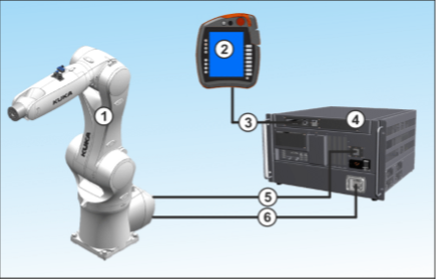
\includegraphics[scale=0.5]{Description_of_KUKA_manipulator}
    	\caption{Description of KUKA arm}
\end{figure}

\section{Warnings and notes}
These warnings are relevant to safety and must be observed.
\begin{figure}[h]
	\centering
	\includegraphics{warning_and_notes}
    	\caption{warning and notes}
\end{figure}


\section{Workspace, safety and danger zone}
Workspaces are to be restricted to the necessary minimum size it must be safeguarded using appropriate safeguards.The safeguard must be situated inside the safety zone. In the case of a stop, the manipulator and external axes are braked and come to a stop within the danger zone which consists of the workspace and the stopping distances of the manipulator.The maximum reach of the robot is 901mm
\begin{figure}[h]
	\centering
	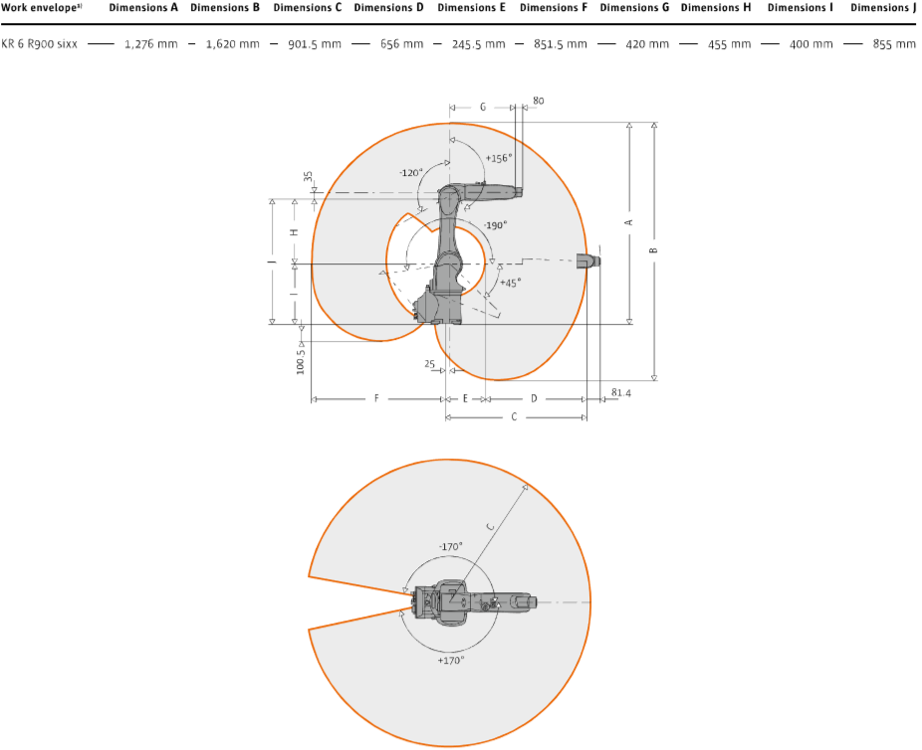
\includegraphics[scale=0.6]{workspace}
    	\caption{Working space}
\end{figure}

\section{Safety function}
\begin{itemize}
    \item Emergency stop is the device must be pressed in the event of a hazardous situation or emergency, The manipulator and any external axes are stopped with a safety stop1.
   
    \item Enabling device of the industrial robot are the enabling switches on the
    KCP.There are 3 enabling switches installed on the KCP which have 3 positions
    \begin{itemize}
        \item Not pressed
        \item Center position
        \item Panic position
	 \end{itemize}
 
 \item Jog mode is an additional protective equipment where the robot use operating modes T1 and T2 to execute the program.This means that it is necessary to hold down an enabling switch and the Start key in order to execute a program.
 
 \item operator safety is a signal used for interlocking physical safety gate in case of losing the signal during automating operation the manipulator will stop with stop 1.
\end{itemize}